\documentclass[a4j]{jarticle} %jsrticleでもいい
\usepackage{fancyhdr} %ヘッダーを表示させるのに必要
\usepackage{listingsutf8}%日本語
\usepackage{color}
\usepackage{comment} %複数行のコメントアウトのパッケージ
\usepackage{amsmath,amssymb}
\usepackage[dvipdfmx]{graphicx}
\usepackage{here}
\usepackage{ascmac}
\usepackage{subfigure}%画像を横に配置
\setlength{\parindent}{0pt}


\pagestyle{fancy}
  \lhead{メディア情報学プログラミング演習} %ヘッダー左
  \rhead{J1-26} %ヘッダー右
\topmargin =-15mm %ページ上部の隙間の調整

\title{令和6年度 メディア情報学プログラミング演習\\グループプログラミング レポート\\料理提供ゲーム「MiniCook」}
\renewcommand{\lstlistingname}{コード}
\begin{document}
\maketitle

\begin{center}%中央に表書く
  \begin{tabular}{|c||c|}
      \hline
      学科&情報理工学域\\
      \hline
      クラス&J1\\
      \hline
      グループ番号&26\\
      \hline
      2210259&米谷祐希\\
      \hline
      2210730&鈴木早紀\\
      \hline
      2210743&吉田陽音\\
      \hline
  \end{tabular}
\end{center}

\newpage

\section{概要説明}
 このゲームは、レストランで働くプレイヤーが、制限時間内に料理を作るゲームである。以下の料理提供までの手順を繰り返すことでポイントを獲得し、制限時間終了時にスコアとランクが表示される。
\begin{enumerate}
  \item オーダーの確認\par
   まず、画面上部にランダムにオーダーが提示される。オーダーには、使う食材と調理方法が記載されている。各オーダーにはそれぞれ制限時間が設定されており、残り時間はオーダー上のゲージにリアルタイムに表示される。
  \item 食材の調理\par
   次に、オーダーに記載されている食材を、各食材ボックスから取り出す。各食材を持ったまま、各調理器具の前でアクションボタンを押すことで、食材が加工される。
  \item 料理の完成と提供\par
   料理は、加工された食材とお皿を組み合わせることで完成する。それらを組み合わせて料理ができあがれば、提供口に置くことで提供となり、オーダーと一致しているか判定される。一致していれば加点、間違っていれば減点となる。   
\end{enumerate}
 また、ゲームは3画面に分かれており、スタート画面、ゲーム画面、リザルト画面がある。また、各画面や各動作にはBGMや効果音がついている。操作はキーボードのA,S,D,W,J,K,Spaceキーを用いている。\par
 作業はGitHubを用い保存・共有を行った。米谷がModelと全体の管理、鈴木がView、吉田がControllerを主に担当したが、最終的には各自の担当領域を超えて協力しながら取り組んだ。


\section{設計方針}
 図1にクラス図を示す。MVCモデルで設計した。%%%%%%%%%%%%%%%%%%%%%%%%%%%%%
\begin{figure}[H]
  \begin{center}
  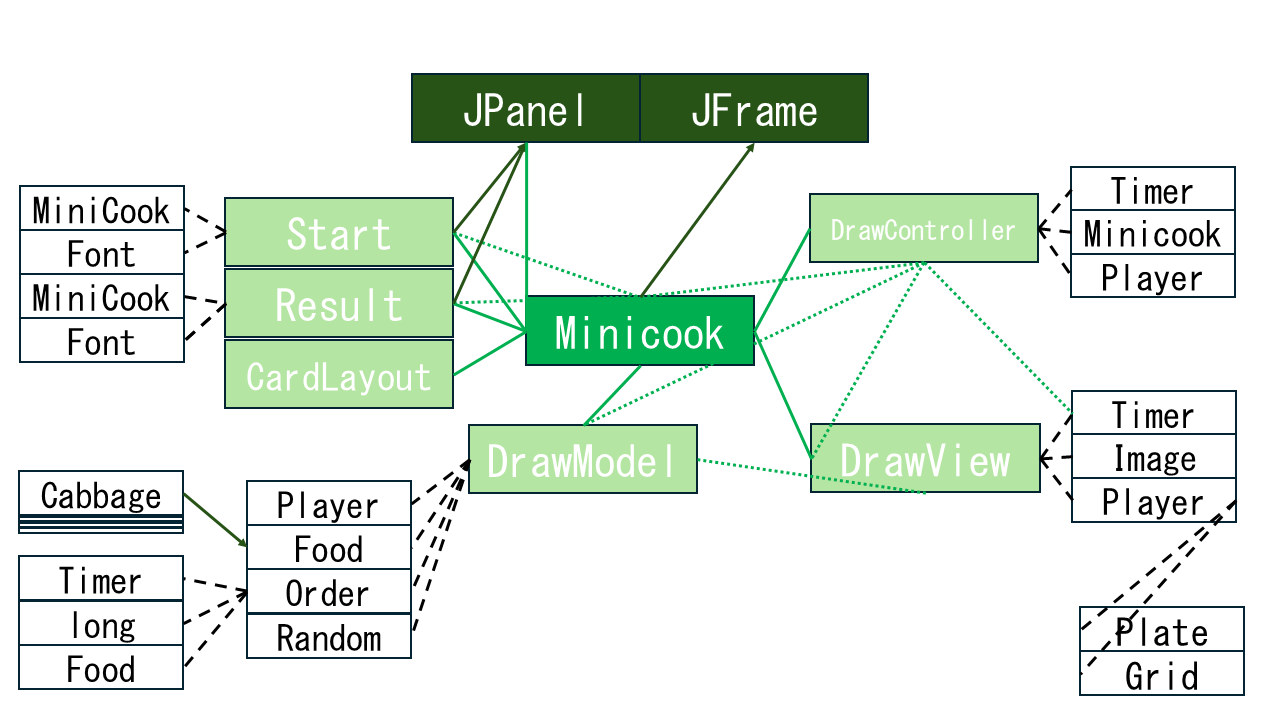
\includegraphics[scale=0.3]{img/class.png}
  \caption{クラス図}
  \end{center}
\end{figure}



\section{プログラムの説明}
 以下にクラスとその説明を示す。
\begin{itemize}
  \item MiniCook\par
   %%%%%%%%%%%%%%%%%%%%%%%%%%%%
  \item Model\par
   %%%%%%%%%%%%%%%%%%%%%%%%%%%
  \begin{itemize}
    \item Food\par
     %%%%%%%%%%%%%%%%%%%%
    \item Order\par
     %%%%%%%%%%%%%%%%%%%%% 
  \end{itemize}   
  \item View\par
   %%%%%%%%%%%%%%%%%%%%%%%%  
  \begin{itemize}
    \item Timer\par
     %%%%%%%%%%%%%%% 
    \item Image\par
     %%%%%%%%%%%%%%%%%%%%%%%%%
    \item Player\par
     %%%%%%%%%%%%%%%%%%%%%%%%%
    \begin{itemize}
      \item Plate\par
       %%%%%%%%%%%%%%%%%%%%%%%%% 
      \item Grid\par
       %%%%%%%%%%%%%%%%%%%%% 
    \end{itemize}   
  \end{itemize}  
  \item Controller\par
   %%%%%%%%%%%%%%%%%%%%%%%%%%% 
  \item Start\par
   %%%%%%%%%%%%%%%%%%%%% 
  \item Result\par
   %%%%%%%%%%%%%%%%%%%%%%%%% 
  \item CardLayout\par
   %%%%%%%%%%%%%%%%%%%%%%%%%%% 
  \item AudioManager\par
   %%%%%%%%%%%%%%%%%%%%%%%%%%%% 
\end{itemize}



\section{実行例}
\subsection*{スタート画面}
 実行すると始めにこの画面(a)が現れる。スタートボタンを押すとゲーム画面:スタート時(c)になる。
\subsection*{リザルト画面}
 ゲーム終了後はこのリザルト画面(b)になる。スコアによってランクが星の数で表される。
\subsection*{ゲーム画面:スタート時}
 スタート時の画面(c)では、食材などは何もなく、オーダーが1つ入るところから開始される。上部にはオーダー、中央にはゲーム部分、下部にはスコアと制限時間を表示している。
\subsection*{ゲーム画面:オーダー}
 画面上部のオーダー(d)では、完成品、必要な食材、加工方法、残り時間が示されている。
\subsection*{ゲーム画面:加工前}
 加工前の食材(e)をボックスから取り出す。
\subsection*{ゲーム画面:加工後}
 調理器具でアクションを行うと加工される。
\subsection*{ゲーム画面:組み合わせ}
 皿の上に各食材を載せると画像がそれに伴い完成品となる。
\subsection*{ゲーム画面:提供}
 完成した料理を提供口に置くと、ホールスタッフが取りに来る。

\begin{figure}[H]
  \begin{center}
    \subfigure[スタート画面]{
      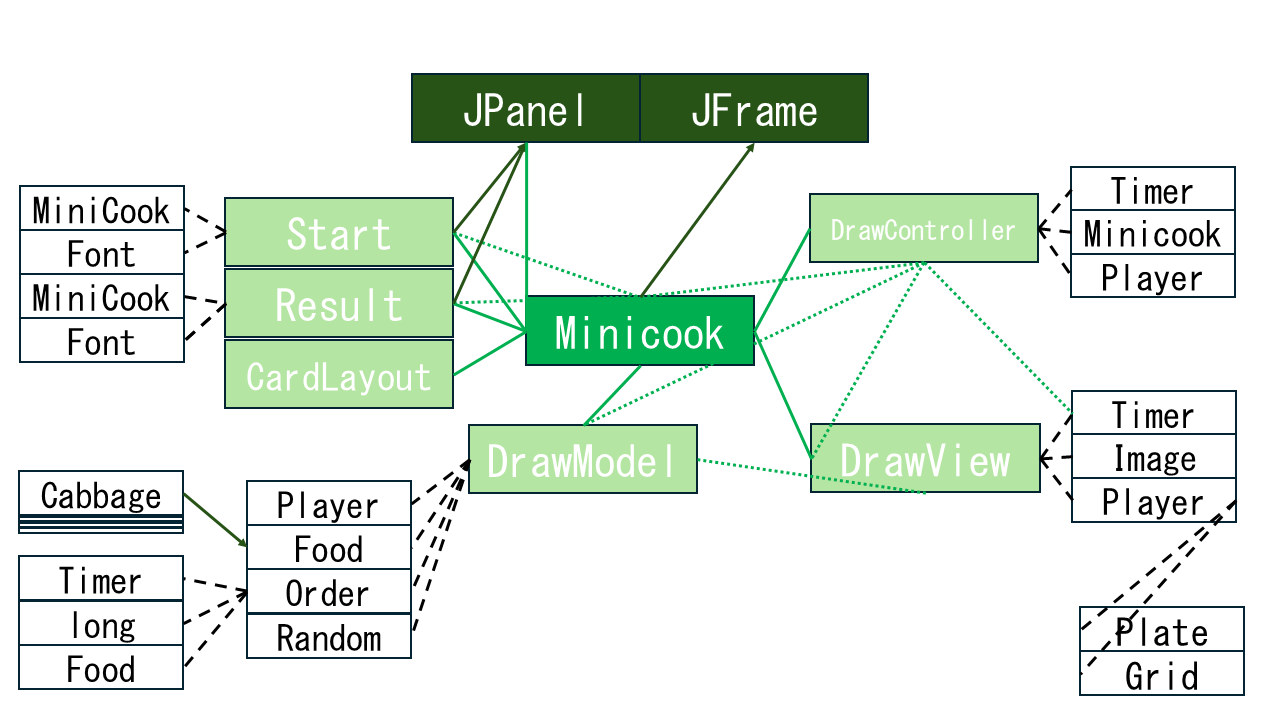
\includegraphics[width=0.4\textwidth,keepaspectratio]{img/class.png}
    }
    \subfigure[リザルト画面]{
      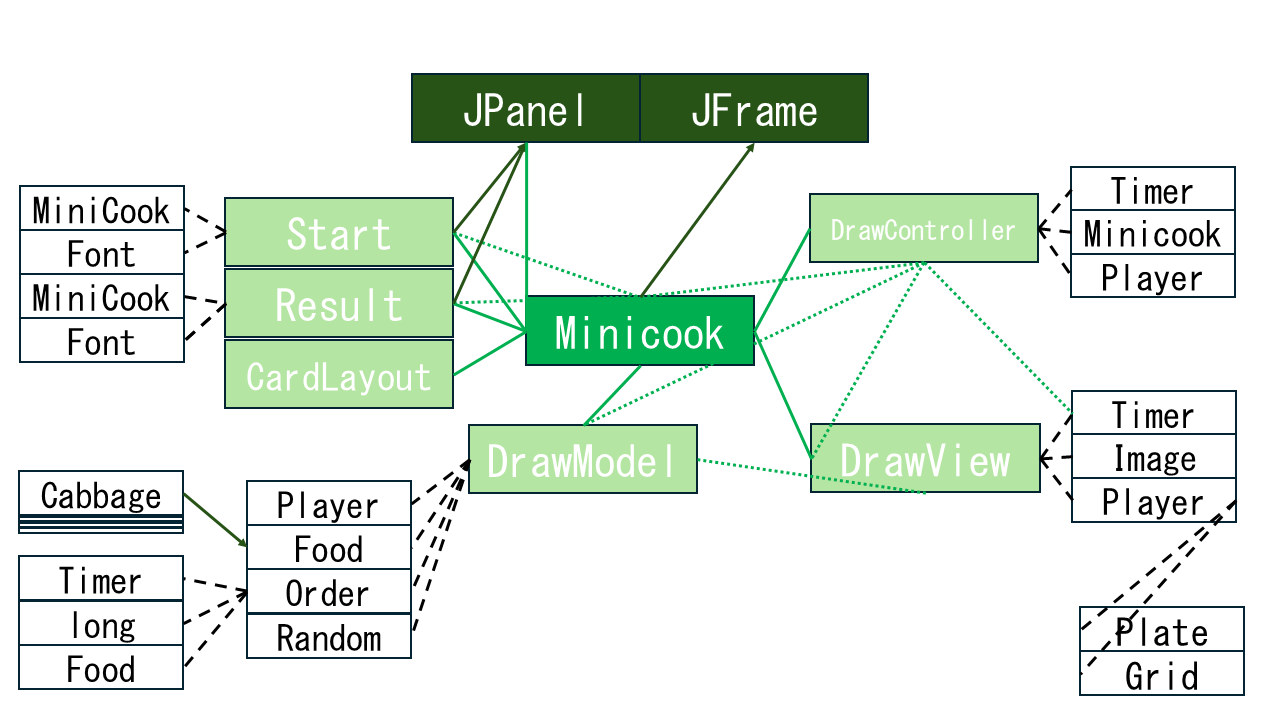
\includegraphics[width=0.4\textwidth,keepaspectratio]{img/class.png}
    }
  \end{center}
\end{figure}
\begin{figure}[H]
  \begin{center}
    \subfigure[ゲーム画面:スタート時]{
      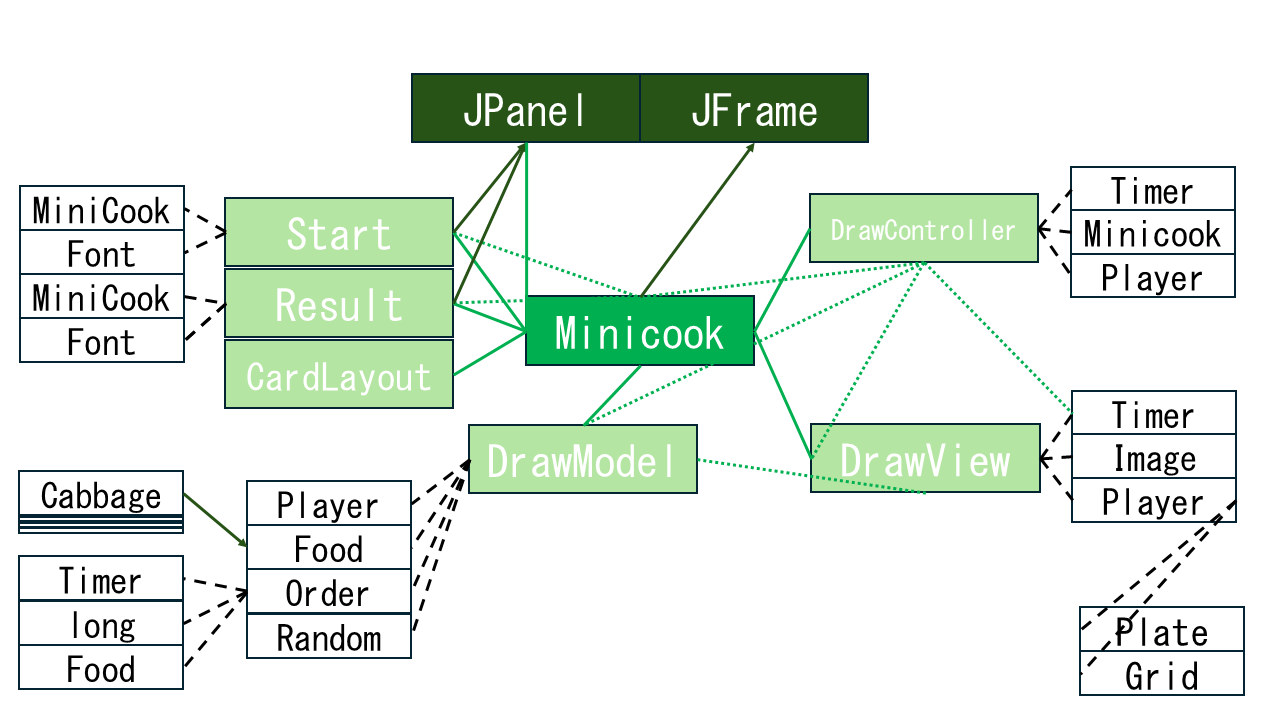
\includegraphics[width=0.4\textwidth,keepaspectratio]{img/class.png}
    }
    \subfigure[ゲーム画面:オーダー]{
      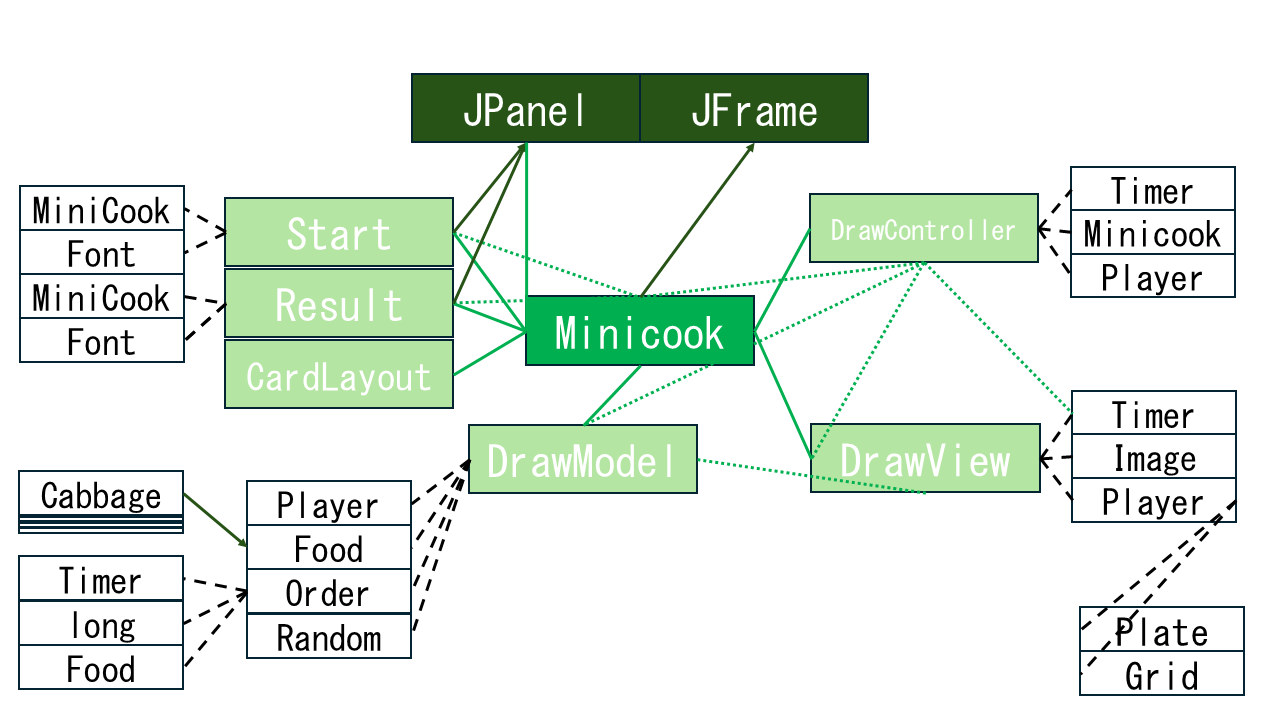
\includegraphics[width=0.4\textwidth,keepaspectratio]{img/class.png}
    }
  \end{center}
\end{figure}
\begin{figure}[H]
  \begin{center}
    \subfigure[ゲーム画面:加工前]{
      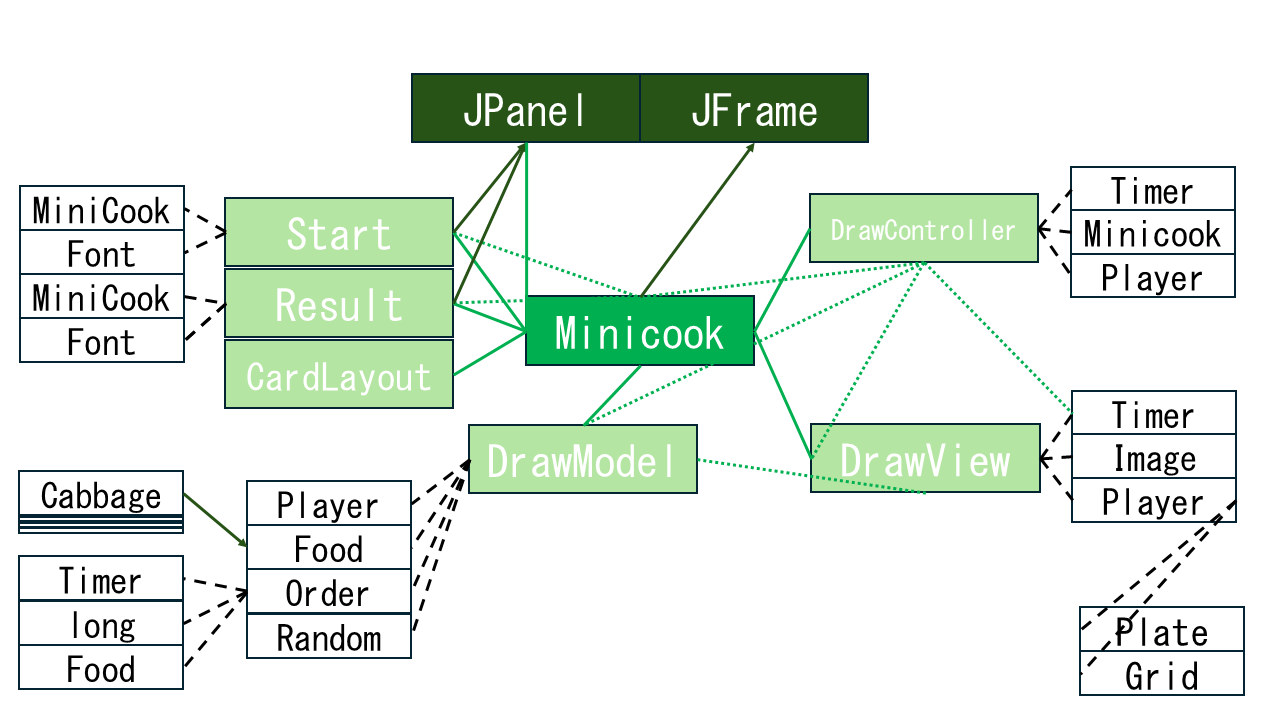
\includegraphics[width=0.4\textwidth,keepaspectratio]{img/class.png}
    }
    \subfigure[ゲーム画面:加工後]{
      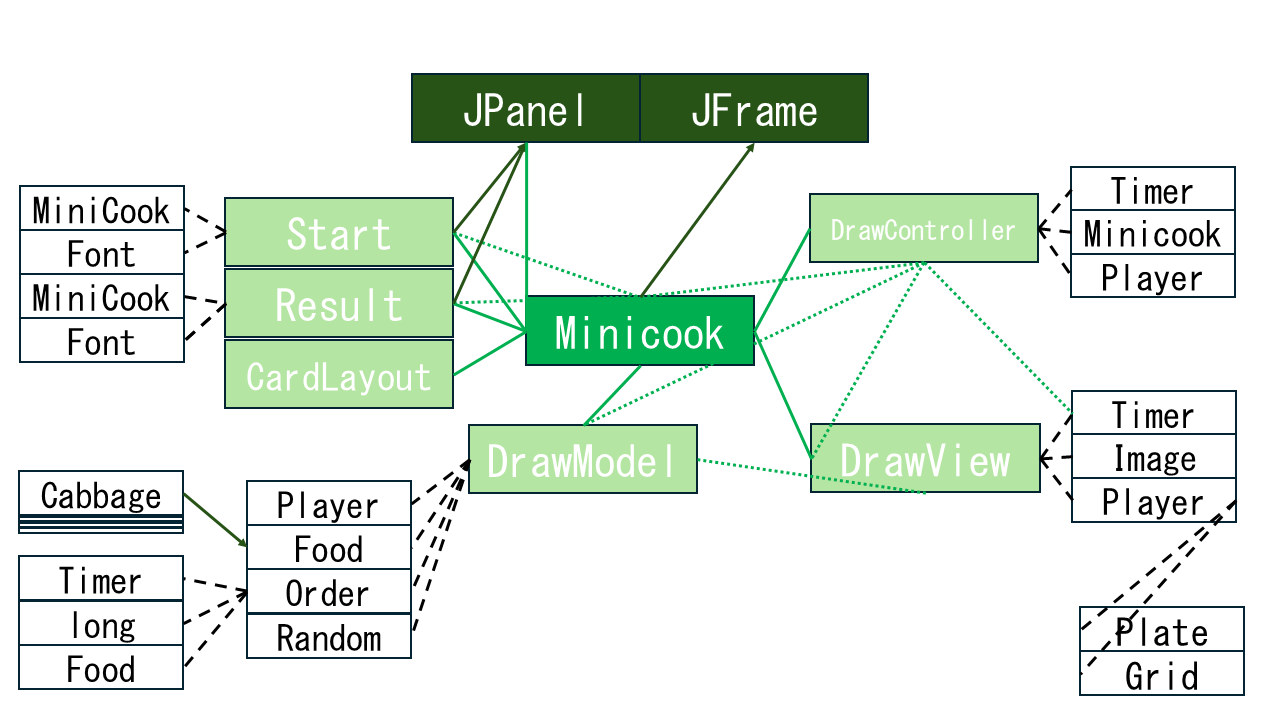
\includegraphics[width=0.4\textwidth,keepaspectratio]{img/class.png}
    }
  \end{center}
\end{figure}
\begin{figure}[H]
  \begin{center}
    \subfigure[ゲーム画面:組み合わせ後]{
      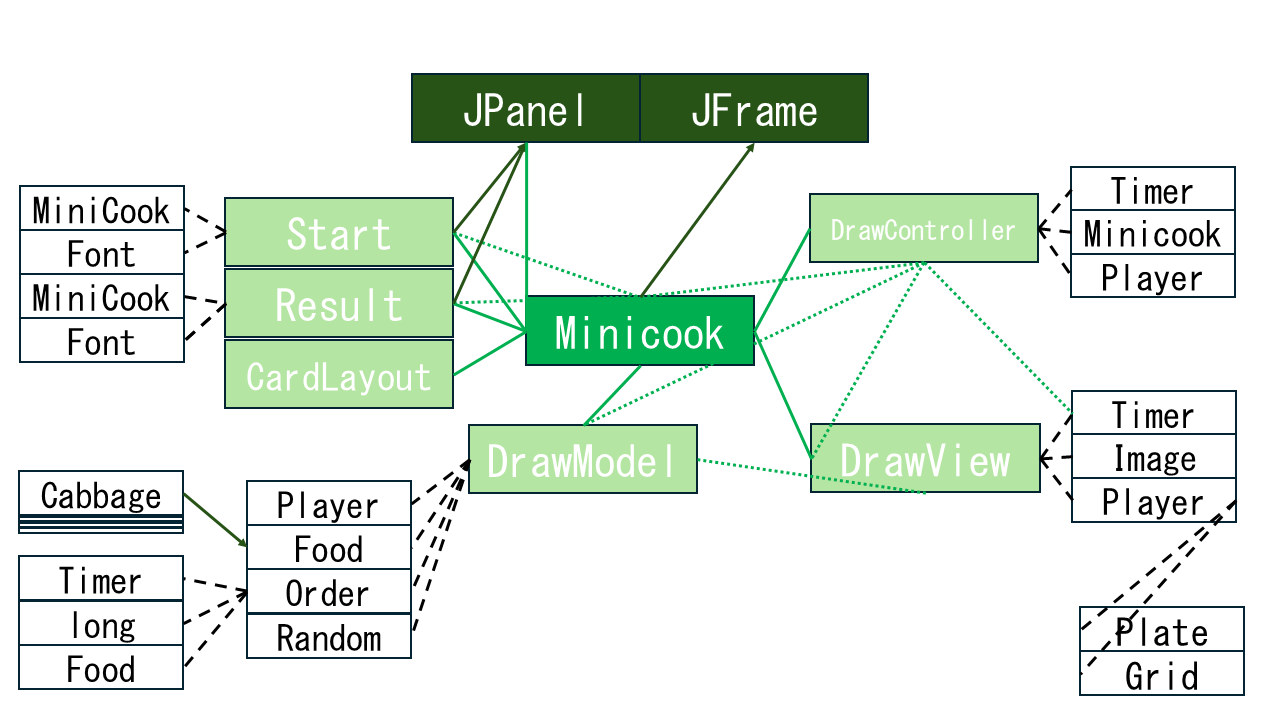
\includegraphics[width=0.4\textwidth,keepaspectratio]{img/class.png}
    }
    \subfigure[ゲーム画面:提供]{
      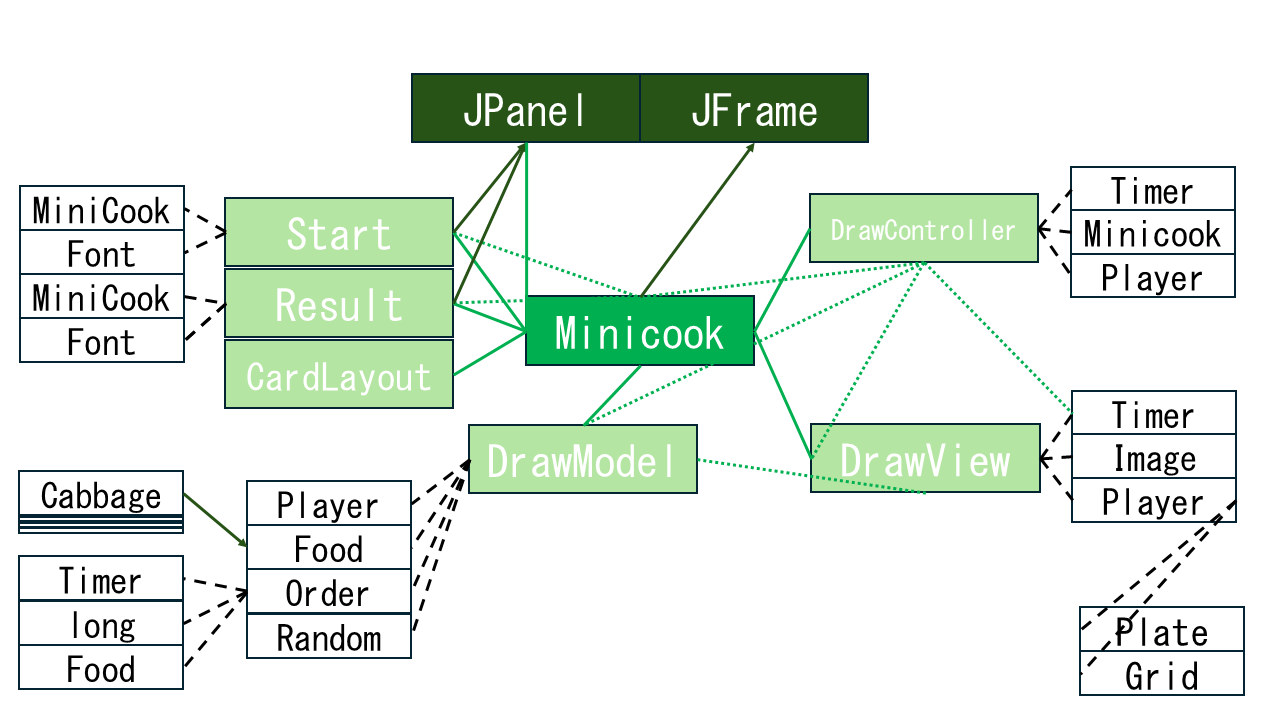
\includegraphics[width=0.4\textwidth,keepaspectratio]{img/class.png}
    }
  \end{center}
\end{figure}

\section{考察}
 予定していた以上のものが完成した。%%%%%%%%%%%%%%%%%%%%%%%

\section{感想}
\subsection*{(米谷祐希)}
 %%%%%%%%%%%%%%%%%%%%%%%%%%%
\subsection*{(鈴木早紀)}
 授業前半の個人の課題を最低限しか取り組まなかったために、2人よりJavaを理解していなくて2人に大変な部分を任せてしまいました。2人が進んで難しいところをやってくれたので感謝しています。画像・音楽の準備やメニューの追加、スライドやレポートは積極的に行えたと思います。2人のプログラムを参考にして理解を進めることができました。今回初めて本格的にグループプログラミングを行ったので、共同作業をする大変さや、作業を分割する便利さを知ることができました。Javaはこの授業で初めて触ったけれど、半年間という期間を考慮すると大きな成果が得られたなと感じます。
%%%%%%%%%%%%%%%%%%%%%%%%%%%%%
\subsection*{(吉田陽音)}
 %%%%%%%%%%%%%%%%%%%%%%%%%%%%


\newpage
\section*{付録1:操作マニュアル}
\subsection*{(ストーリー)}
 キミはレストランのキッチンで働いているぞ!制限時間内にオーダー通りの料理を作れ!目指せ高得点!!
\subsection*{(実行方法)}
 「Java MiniCook」でゲームが開始する。
\subsection*{(操作方法)}
 このゲームはキーボードでキャラクターを操作する。図2にキー操作を示す。W,S,A,Dで上下左右を操作し、Jで取る、Kで置く、スペースキーでアクションを行う。
\begin{figure}[H]
  \begin{center}
  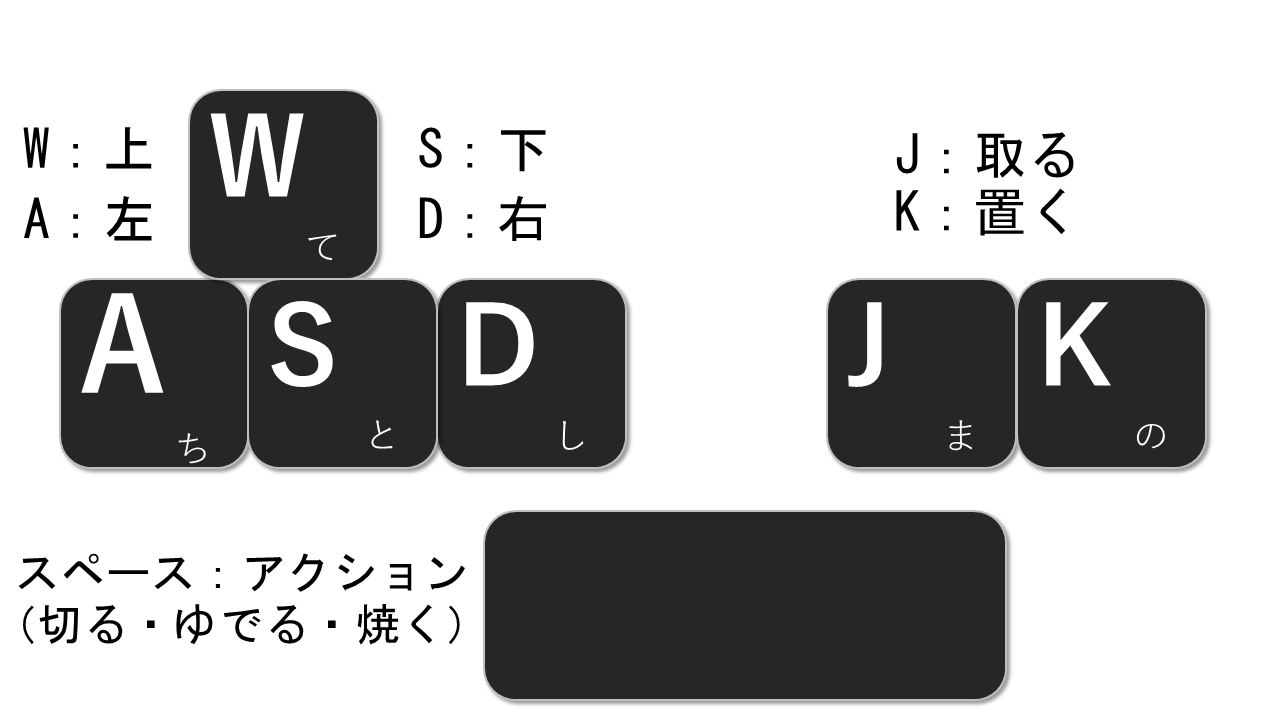
\includegraphics[scale=0.2]{img/key.png}
  \caption{キーボード操作方法}
  \end{center}
\end{figure}
\subsection*{(遊び方)}
\begin{enumerate}
  \item スタート\par
   スタートボタンを押すとゲームが開始する。 
  \item オーダーの確認\par
   まず、画面上部にランダムにオーダーが提示される。オーダーには、使う食材と調理方法が記載されている。各オーダーにはそれぞれ制限時間が設定されており、残り時間はオーダー上のゲージにリアルタイムに表示される。
  \item 食材の調理\par
   次に、オーダーに記載されている食材を、各食材ボックスから取り出す。各食材を持ったまま、各調理器具の前でアクションボタンを押すことで、食材が加工される。
  \item 料理の完成と提供\par
   料理は、加工された食材とお皿を組み合わせることで完成する。それらを組み合わせて料理ができあがれば、提供口に置くことで提供となり、オーダーと一致しているか判定される。一致していれば加点、間違っていれば減点となる。   
  \item リザルト\par
   制限時間がなくなるとリザルト画面に遷移する。スコアとランクが表示される。リザルトを押せばもう一度ゲームが開始する。
\end{enumerate}
\begin{itemize}
  \item メニュー一覧\par
    \begin{itemize}
      \item マグロ握り
      \item イカ握り
      \item 海鮮丼
      \item カッパ巻
      \item 鉄火巻き
      \item サラダ
    \end{itemize}
  \item 調理器具一覧\par
    \begin{itemize}
      \item 包丁
      \item 鍋
    \end{itemize}
  \item 食材一覧\par
    \begin{itemize}
      \item マグロ
      \item イカ
      \item 米
      \item 海苔
      \item キャベツ
      \item トマト
      \item キュウリ
    \end{itemize}     
\end{itemize}



\newpage
\section*{付録2:プログラムリスト}
以下にプログラムリスト全体を記述する。
%%%%%%%%%%%%%%%%%%%%%%%%%%%%%%%%%%%%%%
\lstset{
    language=Java,
    inputencoding=utf8,
    %basicstyle=\ttfamily\scriptsize,
    basicstyle=\ttfamily\tiny,%最小文字、見にくいかも
    extendedchars=false,%日本語のためらしい
    breaklines=true,%長い行折る
    numbers=left,%行番号を左側に
    numberstyle=\tiny,%行番号サイズ
    stepnumber=1, %1行ごとに番号を表示
    frame=single, %枠
    tabsize=4 %タブの幅
}
\begin{itemize}
  \item MiniCook
  \lstinputlisting{../MiniCook.java}
  \item Model
  \lstinputlisting{../Model.java} 
  \item View
  \lstinputlisting{../View.java} 
  \item Controller
  \lstinputlisting{../Controller.java}  
  \item Order
  \lstinputlisting{../Order.java}
  \item Player
  \lstinputlisting{../Player.java}
  \item Start
  \lstinputlisting{../Start.java}
  \item Result
  \lstinputlisting{../Result.java}
  \item Meal
  \lstinputlisting{../Meal.java}
  \item Other
  \lstinputlisting{../Other.java}
  \item AudioManager
  \lstinputlisting{../AudioManager.java} 
\end{itemize}
\normalsize

\end{document}

\begin{comment}
\end{comment}